\section{Implementierung des Backends auf Basis von Alfresco} \label{Implementierung Backend}
F\"ur das Backend eignet sich der Analyse aus Kapitel \ref{Technologievergleich} folgend am besten Alfresco. In den nun folgenden Abschnitten geht es um die Implementierung des Metadatenmodells aus Kapitel \ref{Erstellung eines Datenkonzepts} in Alfresco. Hierf\"ur wird zum einen die Installation und die Arbeitsweise erl\"autert und zum anderen wird im Hauptteil auf die Implementierung des Datenmodells in Alfresco eingegangen.

\subsection{Installation}
Die Installation von Alfresco ist denkbar einfach und unter Windows, sowie unter Linux m\"oglich. F\"ur den Download der Community Edition muss man sich mit einer g\"ultigen E-Mail-Adresse bei Alfresco anmelden, um den Download beginnen zu k\"onnen\footnote{https://www.alfresco.com/de/products/community/download}. 

Die Anmeldung hat den Vorteil, das man zu Webinars und anderen neuen Dingen rund um Alfresco immer auf dem laufenden ist.
Die kostenpflichtige Variante von Alfresco bietet zus\"atzlichen technische Unterst\"utzung und einige Enterprise Features, welche jedoch f\"ur die Arbeit nicht ben\"otigt werden. \cite{Wiki_Alfresco}

Nach dem Download f\"uhrt unter Linux ein Skript die Installation durch. Hierbei wird der Nutzer ausf\"uhrlich \"uber alle getanen Schritte informiert. Der Nutzer muss w\"ahrend der Installation ein Passwort f\"ur das Administrator-Konto "`admin"' angeben.\cite{Alfresco_und_Liferay}

Ist die Installation abgeschlossen und der Server gestartet, kann Alfresco im Browser unter \url{http://127.0.0.1:8080/share/page/} aufgerufen werden. Hier gelangt man zur Anmeldung, wo das bei der Installation angegebene Passwort abgefragt wird.

War die Anmeldung erfolgreich, gelangt der Nutzer auf das "`Administrator Dashboard"', welches in Abbildung \ref{Alfresco Dashboard} im Abschnitten \ref{Alfresco} zu sehen ist.

\subsection{Metadatenmodell in Alfresco} \label{Metadatenmodell von Alfresco}
Um ein Metadatenmodell in Alfresco einf\"ugen zu k\"onnen, muss es mittels XML beschrieben werden. Unter \texttt{ALFRESCO\_HOME} wird im folgenden das Home-Verzeichnis des Alfresco-Servers zu verstehen sein. 

In Abbildung \ref{Alfresco Content-Modell} ist das Content-Modell von Alfresco einmal in UML dargestellt. In der oberen Mitte ist das Hauptelement, die Klasse (Class) zu finden. Eine Klasse beschreibt den Aufbau eines Content-Modells und enth\"alt Aspekte (Aspect) und Typen (Type) welche ganz oben im Diagramm zu sehen sind. \cite{Professional_Alfresco}

Klassen im Content-Modell k\"onnen ihre Eigenschaften, das hei\ss{}t ihre Aspekte und Typen an Unterklassen vererben. In Alfresco ist jedoch nur eine einfache und keien Mehrfachvererbung zul\"assig.

Eine Klasse kann wie um Diagramm gut zu sehen ist entweder Assoziationen auf andere Klassen (Peer Association) oder aber Objekte (Property) enthalten. Eine Assoziationen auf eine andere Klasse ist unter Alfresco jedoch nur zul\"assig, wenn schon ein Kontent der jeweiligen Klasse existiert, andernfalls muss er vorher angelegt werden. Objekte oder auch Attribute k\"onnen aus einem Constraint oder einem einfachen Datentyp (Data Type) bestehen.

Um jedoch das Metadatenmodell wie in Kapitel \ref{Erstellung eines Datenkonzepts} beschrieben umsetzen zu k\"onnen m\"ussen Datentype auch wieder Klassen enthalten k\"onnen. Dies ist jedoch unter keinem \ac{ECM}-Tool m\"oglich. Jedoch bietet Alfresco den besten Ansatz, weshalb das Datenmodells nun nocheinmal f\"ur Alfresco angepasst werden muss. Wie genau das Metadatenmodell angepasst wurde, ist im Abschnitt \ref{Ver\"andertes Datenmodell f\"ur Alfresco} genauer erl\"autert.

Unter Alfresco kann eine Klasse mehrere Typen enthalten, ein Typ kann zum Beispiel ein Bild, eine Gesetz oder \"ahnliches sein. Jeder Typ kann Attribute beinhalten, welche fest mit ihm verbunden sind. Werd eine PDF-Datei in Alfresco also zu einem "`Gesetz"' also zu ein Dokument mit dem Datentyp Gesetz umgewandelt enth\"alt es unweigerlich nach der \"Anderung alle Attribute, welche direkt im Typ beschrieben und verankert sind.

Ein Aspekt kann frei definiert werden und besitzt die M\"oglichkeit sich unabh\"angig vom Typ hinzuf\"ugen zu lassen. M\"ochte ein Nutzer also die Attribute von \ac{INSPIRE} hinzuf\"ugen, so reicht es wenn er den entsprechenden Aspekt zum Dokument hinzuf\"ugt. Vorausgesetzt nat\"urlich, dass die jeweiligen Datentypen als Aspekt definiert sind.

\begin{figure}[!ht]
\centering
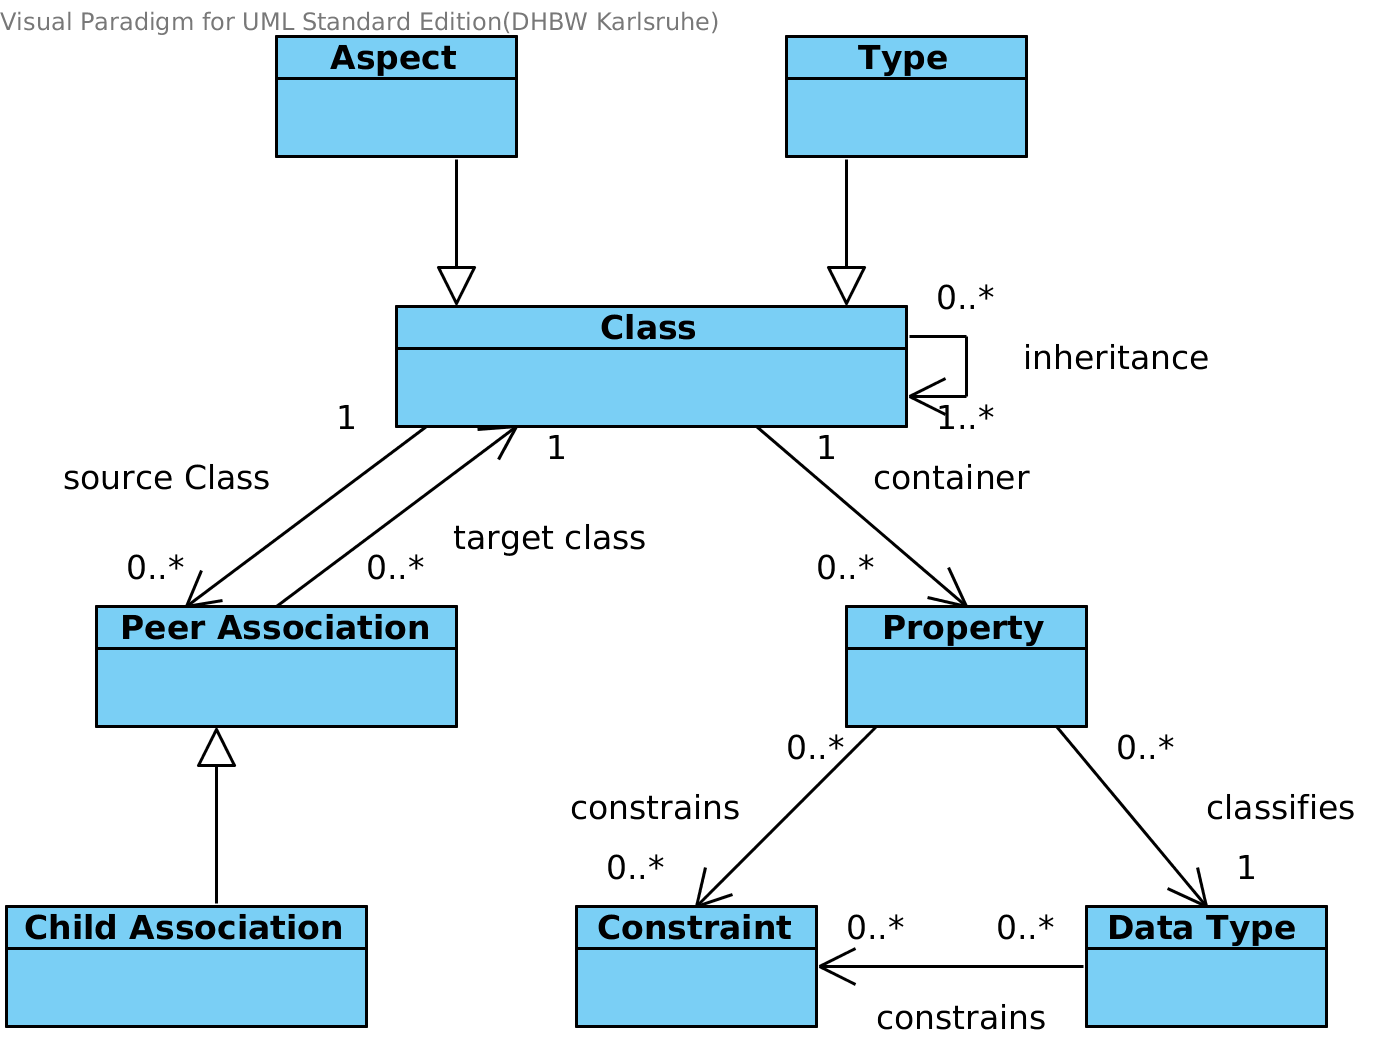
\includegraphics[width=10cm]{Bilder/Alfresco_Contentmodel.png}
\caption{Content-Modell in Alfresco}
\label{Alfresco Content-Modell}
\centering
\end{figure}

\subsection{Ver\"andertes Datenmodell f\"ur Alfresco}\label{Ver\"andertes Datenmodell f\"ur Alfresco}
Wie im Abschnitt \ref{Metadatenmodell von Alfresco} schon ausf\"uhrlich beschrieben, ist es nicht m\"oglich die zuvor im Kapitel \ref{Erstellung eines Datenkonzepts} Metadatenstruktur Eins zu Eins umzusetzen. Daher wird nun beschrieben, wie das Datenmodell f\"ur Alfresco angepasst wurde.

Da Alfresco den "`Dublin Core"'-Standard schon implementiert hat entf\"allt dieser in der Implementierung. Auch die Datensammlung \texttt{Datei} entf\"allt da diese Daten automatisch bei jeder hochgeladenen Datei erstellt werden. 

Die im Abschnitt \ref{FADO Metadaten} gezeigten Datensammlungen werden nun zu Datentypen, welche das jeweilige Dokument beschreiben. Alle farbig hinterlegten Attribute stellen Aspekte dar, die von anderen Klassen aus Alfresco \"ubernommen wurden.

Alle in den folgenden Abschnitten nicht aufgef\"uhrten Datensammlungen sind in den Aspekt direkt untergebracht, da Alfresco wie schon erw\"ahnt eine Klassen, oder Typen als Attribute zul\"asst.

\subsubsection{Die Datentypen}\label{Die Datentypen}
Die in den Abschnitten \ref{FADO Metadaten} bis \ref{ICT-ENSURE Metadaten} gezeigten Grunddatentypen bleiben im angepassten Modell weitestgehend identisch. Da unter Alfresco eine Datei nur von einem Datentyp sein kann, wurde die Datensammlung \texttt{FADO Metadaten} den anderen \ac{FADO}-Sammlungen \"ubergeordnet, wie in Abbildung \ref{Fado Datentypen f\"ur Alfresco} zu sehen ist.

\begin{figure}[!ht]
\centering
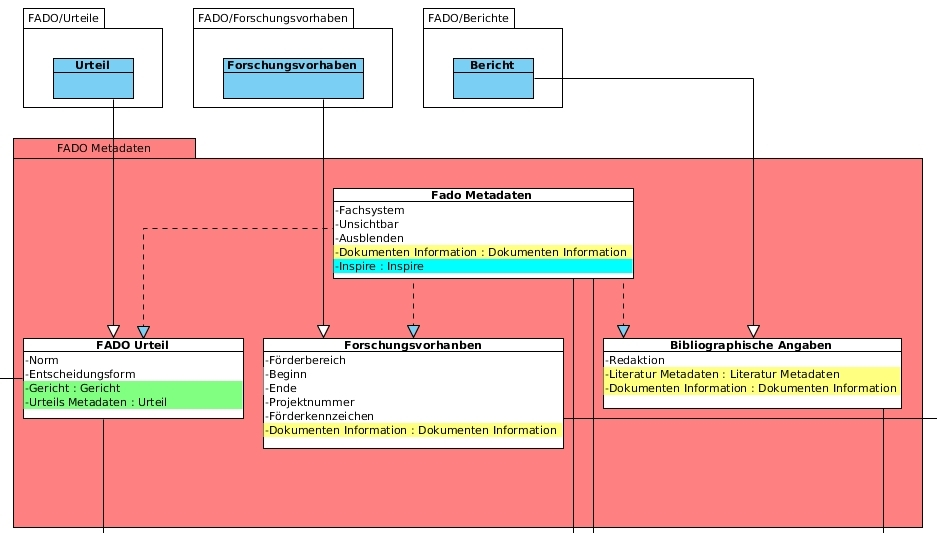
\includegraphics[width=16cm]{Bilder/AlfrescoModell/Fado-Datentypen.jpg}
\caption{FADO Datentypen f\"ur Alfresco}
\label{Fado Datentypen f\"ur Alfresco}
\centering
\end{figure}

Die Datentypen \texttt{DRS-Metadaten} und \texttt{Bildarchiv Metadaten} sind im Grunde gleich geblieben. Hier haben sich nur geringf\"ugige \"Anderungen ergeben, da die Datensammlungen zu wieder Zusammengefasst worden sind. Die beiden Datensammlungen \texttt{Artikel Metadaten} und \texttt{Konferenz} sind zusammengefasst worden und nun im Typ \texttt{Artikel Metadaten} zu finden.
Die eben beschrieben \"Anderungen sind in den Abbildungen \ref{Bildarchiv und ICT-ENSURE Datentypen f\"ur Alfresco} und \ref{DRS Datentyp f\"ur Alfresco}

\begin{figure}[!ht]
\centering
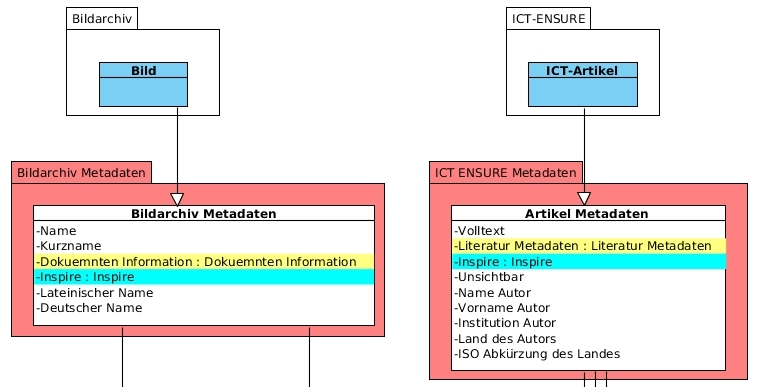
\includegraphics[width=12cm]{Bilder/AlfrescoModell/Bildarchiv-und-ICT-Datentypen.jpg}
\caption{Bildarchiv und ICT-ENSURE Datentypen f\"ur Alfresco}
\label{Bildarchiv und ICT-ENSURE Datentypen f\"ur Alfresco}
\centering
\end{figure}

Im Abschnitt \ref{Die Klasse Gerichtbarkeit} wird noch einmal genauer erw\"ahnt, warum die Attribute \texttt{Fundstelle}, \texttt{Datum Rechtsvorschriften} und \texttt{Ablage} nicht mehr existieren.

\begin{figure}[!ht]
\centering
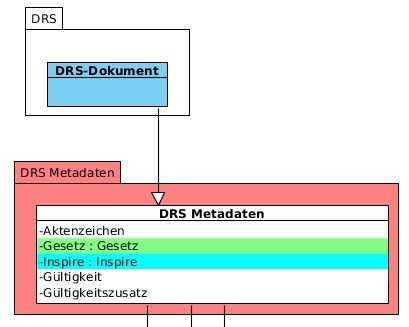
\includegraphics[width=6cm]{Bilder/AlfrescoModell/DRS-Datentypen.jpg}
\caption{DRS Datentyp f\"ur Alfresco}
\label{DRS Datentyp f\"ur Alfresco}
\centering
\end{figure}

\subsubsection{Die Klasse Gerichtbarkeit}\label{Die Klasse Gerichtbarkeit}
Das Package Gerichtbarkeit, beschreibt eine Klasse, welche drei Aspekte beinhaltet. Diese Aspekte sind \texttt{Gesetz}, welcher die Datensammlungen \texttt{Fundstelle}, \texttt{Datum der Rechtsvorschriften} und \texttt{Ablage} zusammengefasst, \texttt{Urtei} und \texttt{Gericht}. 

Die Datensammlung \texttt{Gericht} geht ohne Ver\"anderung einfach in einen Aspekt \"uber und wird im Typ \texttt{FADO Urteil} verwendet. Die Sammlungen \texttt{Urteil} musste etwas abge\"andert werden. Die Verweise Auf das Vorgericht und das Nachgericht wurden aufgeschl\"usselt, da Alfresco bekanntlich keine Klassen als Attribute unterst\"utzt.

In Abbildung \ref{Klasse Gerichtbarkeit} ist die Klasse Gerichtbarkeit noch einmal dargestellt. Zu beachten ist, dass das Package hier f\"ur eine gesamte Klasse steht und die eigentlichen Klassen nur Aspekte darstellen.

\begin{figure}[!ht]
\centering
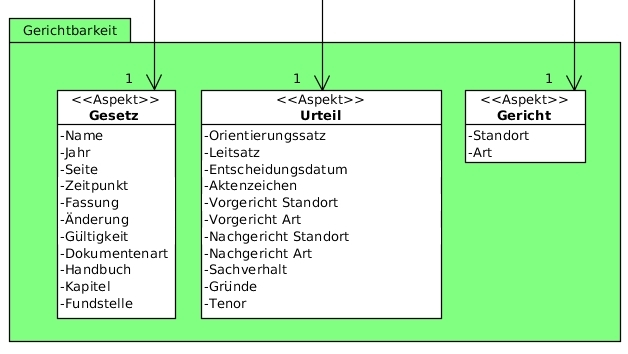
\includegraphics[width=11cm]{Bilder/AlfrescoModell/Gerichtbarkeit.jpg}
\caption{Die Klasse Gerichtbarkeit}
\label{Klasse Gerichtbarkeit}
\centering
\end{figure}

\subsubsection{Die Klasse Standard Aspekte}\label{Die Klasse Standard Aspekte}
Das Package Inspire, ist wieder eine Alfresco Metadaten-Klasse, welche den Aspekt \texttt{Inspire} enth\"alt. Durch die \"Anderungen am Datenmodell, wurden die Attribute, welche sich in den verweisten Datensammlungen befunden haben, nun direkt in der Datensammlung \texttt{Inspire}, welche nun ein Aspekt ist. 

Die Abbildung \ref{Klasse Standard Aspekte} zeigt noch einmal den Aspekt \texttt{Inspire}, welcher sich in der Klasse (dem Package) Standard Aspekte befindet.

\begin{figure}[!ht]
\centering
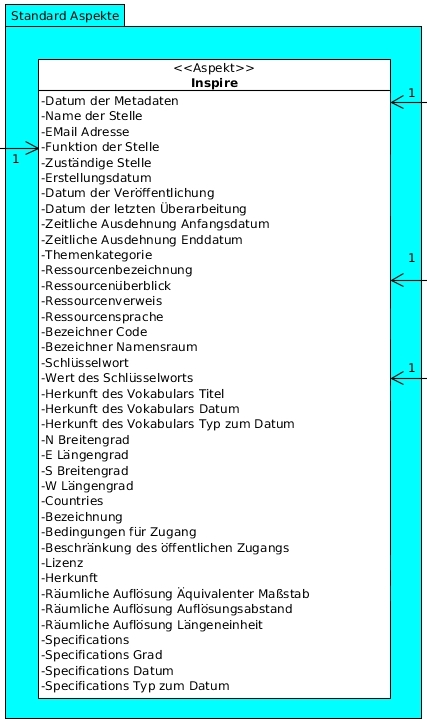
\includegraphics[width=8cm]{Bilder/AlfrescoModell/Standard-Aspekte.jpg}
\caption{Die Klasse Standard Aspekte}
\label{Klasse Standard Aspekte}
\centering
\end{figure}

\subsubsection{Die Klasse Bibliografische Aspekte}
In Abbildung \ref{Klasse Bibligrafische Aspekte} ist die Klasse Bibliografische Aspekte zu sehen, welche die beiden Aspekte \texttt{Dokumenten Information} und \texttt{Literatur Metadaten} enth\"alt.

Beim Aspekt \texttt{Dokumenten Information} ergaben sich keine \"Anderungen, au\ss{}er das das Attribut "`Stand"' nun eigenst\"andig ist und nicht mehr auf ein Datum verweist. Der Aspekt \texttt{Literatur Metadaten} enth\"alt nun die Attribute der Datensammlungen \texttt{Kapitel} und \texttt{Publikations ID}

\begin{figure}[!ht]
\centering
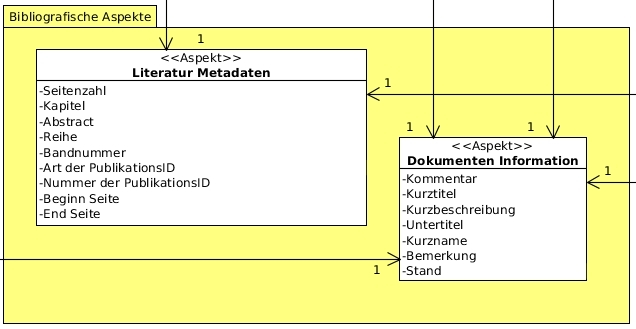
\includegraphics[width=10cm]{Bilder/AlfrescoModell/Bibliografische-Aspekte.jpg}
\caption{Die Klasse Standard Aspekte}
\label{Klasse Bibligrafische Aspekte}
\centering
\end{figure}

\FloatBarrier
\subsection{Implementierung einer Datensammlung}
Eine Datensammlung in Alfresco wird im Verzeichnis \texttt{ALFRESCO\_HOME/tomcat/shared/classes
/alfresco/extensions} abgelegt.
Als Beispiel wird die Datensammlung \texttt{Kontakt f\"ur Metadaten} aus dem Package \texttt{Abstrakte Standard Metadaten} angelegt, welche im Abschnitt \ref{Abstrakte Standard Metadaten} genauer beschrieben wird.

